\documentclass{article}%
\usepackage[T1]{fontenc}%
\usepackage[utf8]{inputenc}%
\usepackage{lmodern}%
\usepackage{textcomp}%
\usepackage{lastpage}%
\usepackage{authblk}%
\usepackage{graphicx}%
%
\title{Essential roles of PI(3)Kp110b in cell growth, metabolism and tumorigenesis}%
\author{Brent Cooper}%
\affil{The Johns Hopkins Oncology Center, Program in Human Genetics, and The Howard Hughes Medical Institute, The Johns Hopkins University School of Medicine, 424 N. Bond Street, Baltimore, 21231, Maryland, USA}%
\date{01{-}01{-}2011}%
%
\begin{document}%
\normalsize%
\maketitle%
\section{Abstract}%
\label{sec:Abstract}%
The false negatives in the Mitchell Collection of twins present evidence of an MITF{-}defective mutations in mitochondria, a group of low{-}power and specialized body cells that are important for maintaining a healthy cell surface area and responding to synthetic chemicals in their environment. These false negatives were identified by Harvard colleague Francis Chan as potential culprits in a 1998 mitochondrial genome correction study.\newline%
In 2010, a new study in the Proceedings of the National Academy of Sciences indicates that this false negative Mitochondrial gene mutation is also associated with kidney and liver tumors, prostate and kidney cancer, colon and rectal cancer, and tumors of the esophagus. Many other mutations also exist which cause abnormal cellular activity, disrupting the internal structure and function of the mitochondria. The Mitochondrial gene mutation mutations in these genetic abnormalities that lead to these diseases are the result of mutations in other known genes or potentially defective genes in many genes. Thus, genetic mutations in genes which are generally considered useful to protect against certain types of cancers is not surprising.\newline%
The Mitochondrial gene mutation discovery has implications for how to wean themselves off the danger of the destabilizing (and potentially fatal) compounds that are transforming mitochondria in favor of a more balanced diet and a more active immune system. Ideally, mitochondrial diseases can be treated, corrected, and overcome with simple lifestyle changes, such as avoiding food rich in tumors of the esophagus or kidneys.

%
\subsection{Image Analysis}%
\label{subsec:ImageAnalysis}%


\begin{figure}[h!]%
\centering%
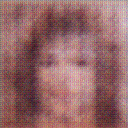
\includegraphics[width=150px]{500_fake_images/samples_5_459.png}%
\caption{A Close Up Of A Person Wearing A Tie}%
\end{figure}

%
\end{document}